\documentclass{article}

\usepackage{graphicx}
\usepackage{tikz}
\usepackage{tikzsymbols}
\usetikzlibrary{calc,patterns,shapes.geometric}
\pagestyle{empty}
\usepackage[margin=0pt]{geometry}
\geometry{papersize={14in,12in}}

\def\centerarc[#1](#2)(#3:#4:#5){\draw[#1] ($(#2)+({#5*cos(#3)},{#5*sin(#3)})$) arc (#3:#4:#5);}

\begin{document}
	\begin{figure}
		\centering
		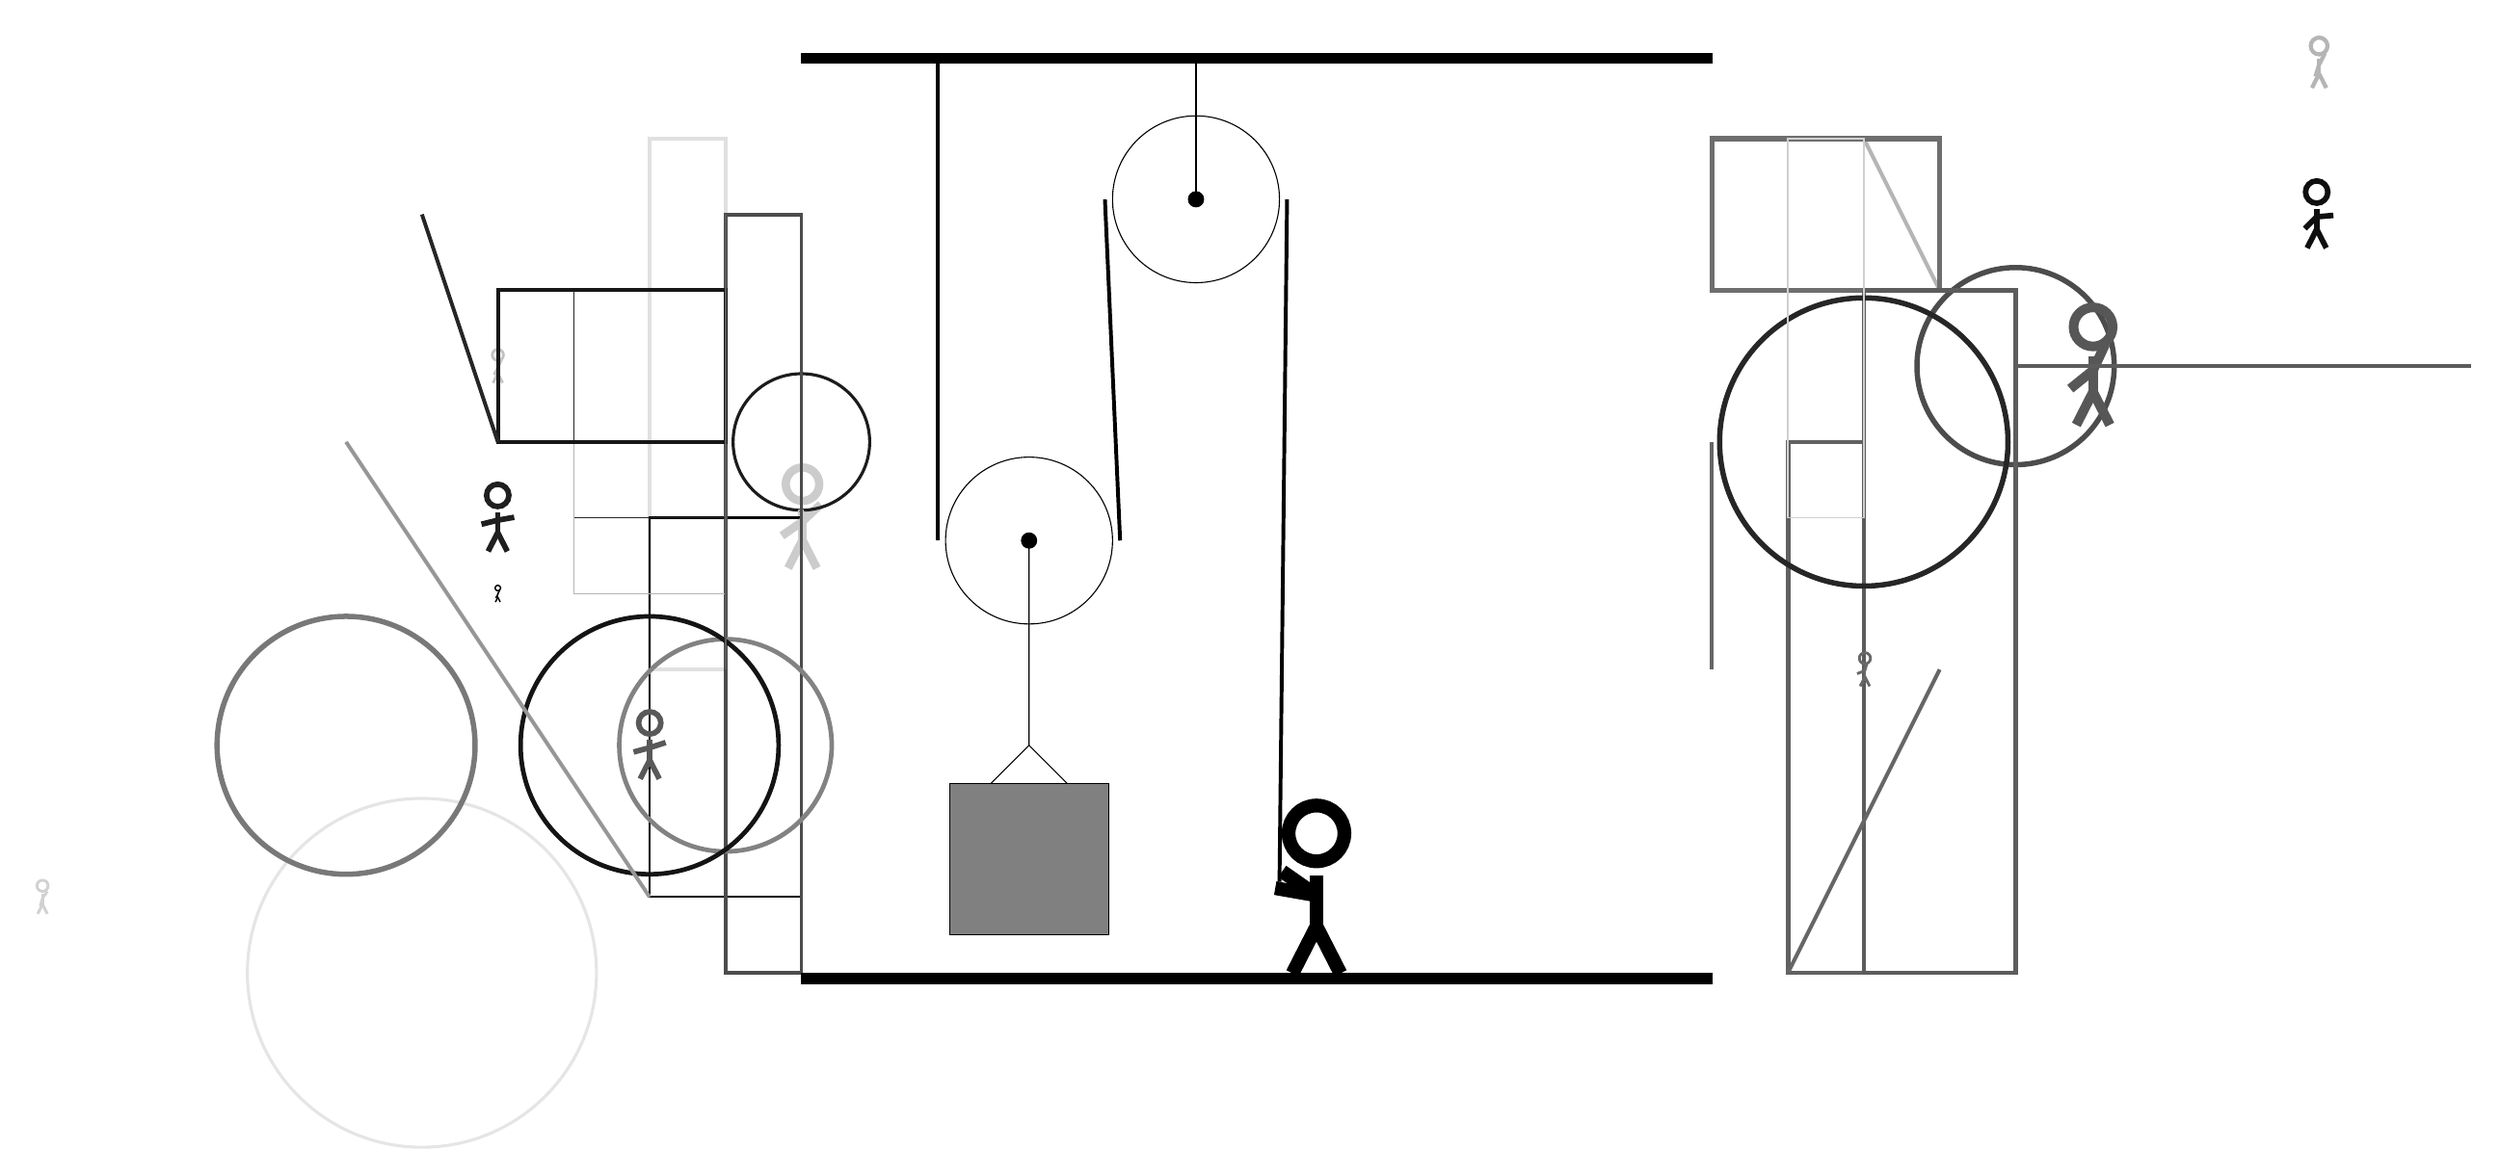
\begin{tikzpicture}
			%%%%% START %%%%%
			
			\draw[fill=black] (-2, 9) rectangle (10, 9.125);
			
			\draw (3.2, 7.2) circle (1.1);
			\draw[fill=black] (3.2, 7.2) circle (0.1);
			\draw[thick] (3.2, 7.2) -- (3.2, 9);
			
			\draw (1, 2.7) circle (1.1);
			\draw[fill=black] (1, 2.7) circle (0.1);
			
			\draw (1, 2.7) -- (1, 0) -- (0.5, -0.5);
			\draw (1, 0) -- (1.5, -0.5);
			\draw[fill=black!50] (-0.05, -0.5) rectangle (2.05, -2.5);
			
			\draw[line width=0.5mm] (-0.2, 9) -- (-0.2, 2.7);
			\centerarc[line width=0.5mm](1, 2.7)(180:360:1.2000000000000002);
			\draw[line width=0.5mm](2.2, 2.7) -- (2.0, 7.2);
			\centerarc[line width=0.5mm](3.2, 7.2)(0:180:1.2000000000000002);
			\draw[line width=0.5mm](4.4, 7.2) -- (4.3, -1.8);
			
			\node at (4.7, -1.9) {\Strichmaxerl[10][-35][170]};
			
			\draw [line width=0.7mm, color=black!70](14, 5) circle (1.3);
			
			\draw[line width=0.5mm, color=black!12] (-4, 1) rectangle (-3, 8);
			\draw[line width=0.5mm, color=black!29](13, 6) -- (12, 8);
			\draw[line width=0.5mm, color=black!60](10, 1) -- (10, 4);
			\node[line width=0.6mm, color=black!66] at (15, 5) {\Strichmaxerl[7][39][65]};
			\node[line width=0.7mm, color=black!20] at (-2, 3) {\Strichmaxerl[6][35][43]};
			
			\node[line width=0.6mm, color=black!29] at (18, 9) {\Strichmaxerl[3][73][63]};
			\draw[line width=0.7mm, color=black!57] (10, 8) rectangle (13, 6);
			\node[line width=0.2mm, color=black!24] at (-6, 5) {\Strichmaxerl[2][64][64]};
			\draw [line width=0.4mm, color=black!89](-2, 4) circle (0.9);
			
			\draw[line width=0.3mm, color=black!98] (-4, -2) rectangle (-2, 3);
			\node[line width=0.5mm, color=black!65] at (-4, 0) {\Strichmaxerl[4][15][18]};
			\node[line width=0.2mm, color=black!94] at (18, 7) {\Strichmaxerl[4][45][5]};
			\draw[line width=0.6mm, color=black!62] (12, 4) rectangle (11, -3);
			\node[line width=0.2mm, color=black!21] at (-2, 3) {\Strichmaxerl[1][40][14]};
			\node[line width=0.5mm, color=black!18] at (-12, -2) {\Strichmaxerl[2][74][55]};
			\node[line width=0.5mm, color=black!88] at (-6, 3) {\Strichmaxerl[4][14][10]};
			
			\draw [line width=0.4mm, color=black!10](-7, -3) circle (2.3);
			\draw[line width=0.5mm, color=black!14] (12, 3) rectangle (12, 0);
			\draw[line width=0.5mm, color=black!70] (-2, 7) rectangle (-3, -3);
			\draw[line width=0.6mm, color=black!64] (12, -3) rectangle (14, 6);
			
			\draw[line width=0.5mm, color=black!60](11, -3) -- (13, 1);
			
			\draw[line width=0.2mm, color=black!85] (-3, 3) rectangle (-5, 6);
			\node[line width=0.3mm, color=black!59] at (12, 1) {\Strichmaxerl[2][21][75]};
			\draw [line width=0.6mm, color=black!49](-3, 0) circle (1.4);
			
			\draw[line width=0.2mm, color=black!29] (-3, 2) rectangle (-5, 4);
			\draw [line width=0.6mm, color=black!92](-4, 0) circle (1.7);
			\draw[line width=0.5mm, color=black!91] (-3, 6) rectangle (-6, 4);
			\draw[line width=0.5mm, color=black!85](-6, 4) -- (-7, 7);
			\node[line width=0.7mm, color=black!100] at (-6, 2) {\Strichmaxerl[1][61][66]};
			\draw [line width=0.7mm, color=black!85](12, 4) circle (1.9);
			
			\draw[line width=0.5mm, color=black!41](-4, -2) -- (-8, 4);
			\draw[line width=0.2mm, color=black!19] (12, 8) rectangle (11, 3);
			\draw[line width=0.2mm, color=black!64] (-3, 1) rectangle (-3, 7);
			\draw [line width=0.7mm, color=black!53](-8, 0) circle (1.7);
			\draw[line width=0.5mm, color=black!64](14, 5) -- (20, 5);
			
			
			\draw[fill=black] (-2, -3) rectangle (10, -3.15);
			
			%%%%% END %%%%%
		\end{tikzpicture}
	\end{figure}	
\end{document}